
\documentclass{classes/report}

\usepackage{blindtext}
\usepackage{titlesec}

\setcounter{secnumdepth}{3}

%\title{Determining Molar Enthalpy and Entropy of Vaporization for Acetone and n-Hexane}
\title{Measuring conductivity of water, sodium carbonate and potassium carbonate solutions under varying conditions}

\assistant{Toutoudaki Eirini}{eirini.toutoudaki@phys.chem.ethz.ch}

\authors{Janosch Jörg}{jjoerg@ethz.ch}{DCHAB}{Maria Zimmermann}{mazimmerm@ethz.ch}{DCHAB}

\abstract{}

\begin{document}

    \maketitle
    \newpage
    
    \begin{multicols}{2}
    
        \section{Introduction}
    
            \input{parts/introduction.tex}
            
        %\newpage    
        
        
            
%Characterize the system, give all details that matter. Describe how the experimental procedure went.

% CAS codes Hinzufügen?

\subsection{Chemicals}
The following experiments were conducted using acetone (\qty{58.8}{\gram\per\mole}), from \texttt{Sigma Aldrich}, puriss. p.a., ($\geq$\qty{99.5}{\percent}), n-hexane (\qty{86.18}{\gram\per\mole}), from \texttt{Sigma Aldrich}, ($\geq$\qty{95}{\percent}) and methanol (\qty{32.04}{\gram\per\mole}), from \texttt{VWR Chemicals}, ($\geq$\qty{99.5}{\percent}). All chemicals were used forgoing any further purification.

\subsection{Procedure}
A total of 3 experiments were prepared and carried out as follows:

\subsubsection{Verification}

The identity and purity of acetone and n-hexane were verified by determining their respective \textit{refractive index} and \textit{density}. 

Refractive index measurements were done via digital refractometer \texttt{ATAGO RX-5000} operating at standard wavelength of \qty{589.0}{\nano\meter} (D-line) and with samples maintained at a constant \qty{20.00 \pm 0.02}{\celsius} by a \texttt{LAUDA E100} circulation thermostat (attached to the refractometer). After ensuring the glass surface of the sample block was dry, a small amount of liquid was applied – just enough to cover the circular surface – and once equilibration was reached as indicated by the temperature display, measurements could be initiated.

Density was determined in two different ways.

First, by \textit{method A}, filling a \qty{25.00 \pm 0.04}{\milli\liter} volumetric flask (insert marke) with either liquid and measuring its mass using a \texttt{METTLER-TOLEDO AG204 Delta Range} analytical balance, the accuracy range of which is stated as \qty{0.1}{\milli\gram} by the manufacturer.

And secondly, by \textit{method B}, using an \texttt{ANTON PAAR DMA 48} density gauge (Fig. \ref{fig:sketch_rho}), where the respective sample was carefully inserted via plastic syringe and – after visual confirmation that there were no air bubbles inside the u-shaped glass tube – run at setting \mintinline{R}{F505}. Between measurements of different samples, the tube was rinsed with deionized water and dried by inducing airflow.

\begin{figure}[H]
    \centering
    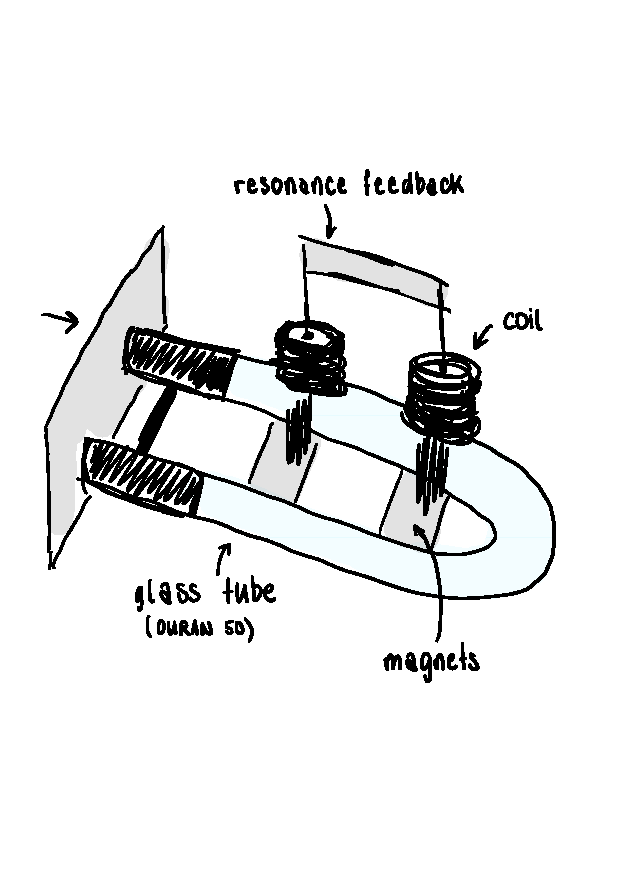
\includegraphics[width=.5\textwidth]{figures/sketch_density_meter.pdf}
    \caption{The \texttt{ANTON PAAR DMA 48} density gauge measures a liquid's density by oscillating a glass tube. The resonant frequency of the glass tube is directly correlated to the liquid's density.}
    \label{fig:sketch_rho}
\end{figure}


%\newpage

\subsubsection{Vapor Pressure}

\begin{figure}[H]
    \centering
    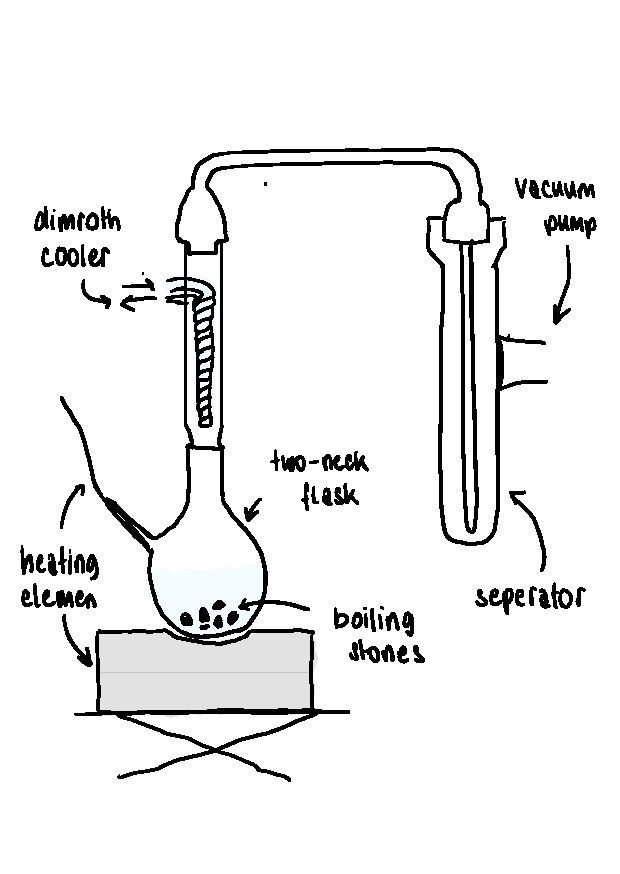
\includegraphics[width=.5\textwidth]{figures/ddr_sketch_setup.pdf}
    \caption{The vapor pressure measurement setup allows temperature and pressure to be controlled while observing the phase transition of the liquid. The temperature was recorded with a thermocouple type K inside the two-neck flask. To adjust the pressure, the vacuum system was connected to a variable needle valve to allow outside air to vent the system.}
    \label{fig:sketch_setup}
\end{figure}

The boiling temperatures of acetone and n-hexane were measured at different pressure settings. 

For this purpose, a two necked flask containing the sample and about 10-15 boiling stones and filled to approximately half its capacity was attached to a pre-prepared setup (Fig.\ref{fig:sketch_setup}), omitting grinding grease due to the risk of contaminating the sample and comparatively low significance of a tight seal in this experiment.

Only after ensuring that all openings were closed, the \texttt{BÜCHI VAC V-503} vacuum pump, dimroth condensation cooler and \texttt{WINKLER WHLG2} laboratory heating mantle with a \texttt{WL10} heating controller were turned on. It is important to note that forgoing the former here and starting the cooler before sealing the system would allow water vapor from the air to condense inside the cooler and likely lead to falsified results. 

While maintaining a low heat supply via the controllable heating mantle, pressure within the system was steadily decreased under close surveillance through evacuation by means of a \texttt{BÜCHI I-100} vacuum controller and a ventilation valve until about \qty{150}{\milli\bar} and \qty{100}{\milli\bar} were reached for acetone and n-hexane respectively and the liquid was simultaneously boiling inside the flask and dripping steadily from the cooler. For acetone we could not observe any dripping at first, yet the liquid seemed to be boiling and the temperature was quickly decreasing to under \qty{10}{\celsius}. We concluded that the vapor currently forming would be at a lower temperature than the liquid in the dimroth cooler, causing it to escape into the separator instead of condensing. As such we increased our heat supply and not long after, equilibrium returned to the system and steady dripping could be observed. 

The temperature measured by the \texttt{GREISINGER GMH 3210} digital temperature gauge (with a resolution of \qty{0.1}{\kelvin}) was marked down with its corresponding vapor pressure and the pressure was incremented in \qtyrange{25}{50}{\mbar} steps until reaching \qty{900}{\mbar}, waiting for the temperature to level out after each increase and recording respective values. This was repeated at decreasing pressure, generating two sets of values for each sample.

%\newpage

\subsubsection{Evaporation Cooling}

\begin{figure}[H]
    \centering
    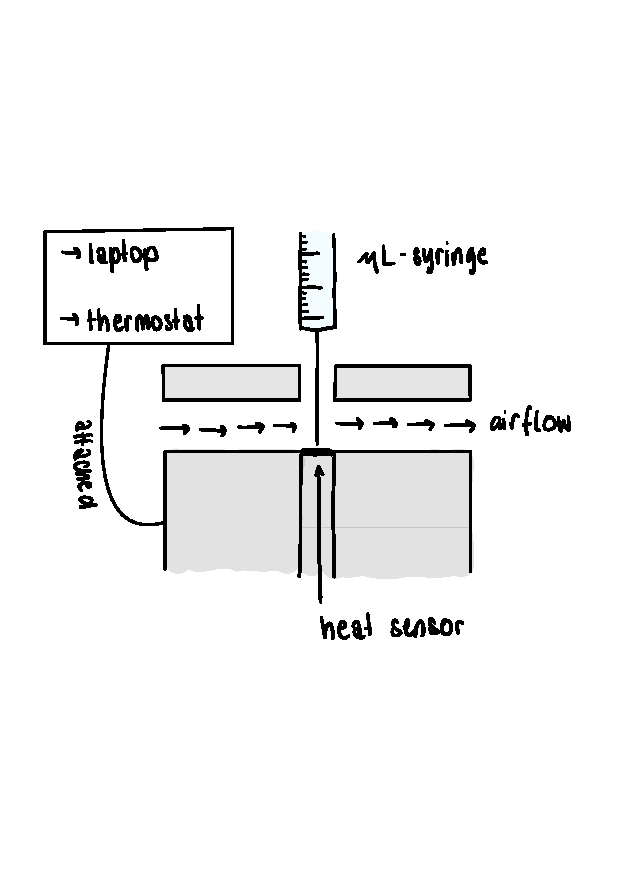
\includegraphics[width=.5\textwidth]{figures/ddr_sketch_TREVAC.pdf}
    \caption{The \texttt{TREVAC} evaporation cooling measurement system causes the liquid to evaporate and draw heat from the sensor plate, resulting in a temporary temperature drop.}
    \label{fig:sketch_trevac}
\end{figure}


The evaporation cooling effect of acetone, n-hexane and methanol (reference sample) were visualized and recorded by measuring the surface temperature of an ultra-sensitive heat sensor at \qty{0.25}{\second} intervals during the evaporation of a predefined volume of liquid sample applied to the sensor.

The setup, a \texttt{TREVAC}-apparatus (transient evaporation cooling) as can be seen in Fig. \ref{fig:sketch_trevac}, self-developed by the \texttt{PCL} at \texttt{ETH Zürich}, relies on a \texttt{LAUDA Ecoline 103} thermostat to keep the aluminium block with the \texttt{NATIONAL LM 35} heat sensor at its center at a programmable base temperature of 

$T_0=$ \qty{35}{\celsius}, 
\\deviating less than \qty{\pm 0.01}{\kelvin}. $T_0$ was selected at \qtyrange{30}{40}{\kelvin} below the boiling point of the lowest-boiling liquid. The sample was inserted at a steady pace via a \texttt{HAMILTON 801 RN} microliter syringe (scale facing forward to ensure measurement circumstances were as similar as possible for each sample inserted), using a measuring gauge to measure out exactly \qty{5}{\micro\liter} and discard any excess liquid beforehand. 

The registered surface temperature over time was recorded via analog/digital converter (ADC, 23 bit) and broadcast on the display of a laptop attached to the setup. A custom LabVIEW program allowed redording and saving the temperature and meta data.

This process was repeated 3 times per substance, leaving enough time for the sensor to equilibrate back to $T_0$ between the end of each prior evaporation and insertion of the current sample.

        
            

\section{Results and Discussion}
The analysis and calculations were conducted using the R programming language \cite{R} and Python Jupyter Notebooks \cite{IPython:2007}. The scripts are included in the appendix of this report. \ref{r_scripts} All uncertainties stated are provided for a 95 \% confidence interval. The uncertainties were modelled with the aid of \texttt{METAS UncLib}, a Python uncertainty modelling library by the Swiss institute of metrology METAS.\cite{unclib}


\subsection{Conductivity of differently treated water samples}

For the different types of water specific conductivities were found to be:

\begin{table}[H]
\centering
\begin{tabular}{
    l
    l
}
\hline
water treatment & $\kappa$ / \textmu S/cm \\ \hline
tap             & 283(14)  \\
deionized       & 2.85(12) \\
degased         & 1.1(3)   \\ \hline
\end{tabular}
\caption{Specific conductivities $\kappa$ of differently treated water samples.}
\end{table}

The measured specific conductivity for the purified, degassed water exceeds the manufacturer specifications of \qty{0.055}{\micro\spc} by a substantial amount.\cite{huber} To accurately measure such low conductivities, a closed measurement apparatus, where no oxygen is absorbed, would be required.



\subsection{Correlation between temperature and conductivity}

The thermal coefficient of the potassium carbonate conductivity was found to be $\alpha_{\mathrm{K_2CO_3}} =$ \qty[per-mode=reciprocal]{0.02143 \pm 0.00008}{\per\kelvin}, and thus closely matching the approximately \qty[per-mode=reciprocal]{0.02}{\per\kelvin} typical for aqueous solutions.\cite{meister} The conductivity at standard conditions was determined at $\kappa(\qty{25}{\celsius}) =$ \qty{19.58 \pm 0.06}{\milli\spc}.

\begin{figure}[H]
    \centering
    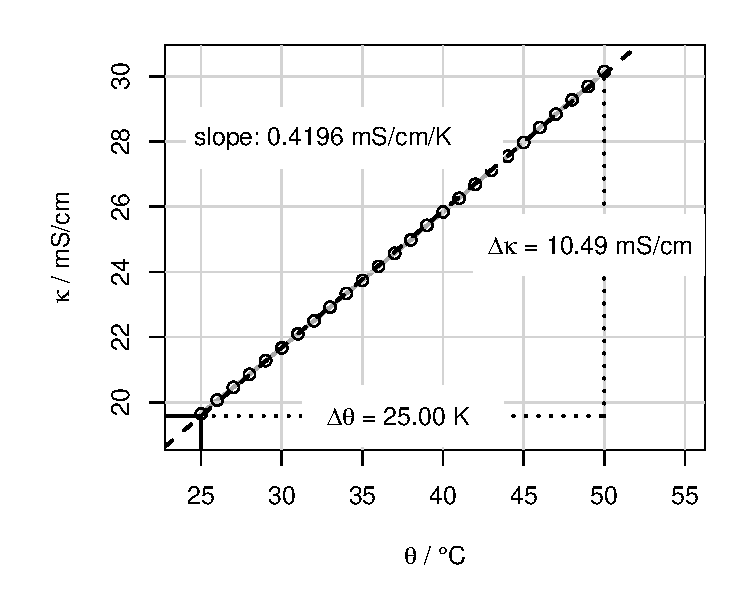
\includegraphics[width=.45\textwidth]{figures/plots/lfk_temperature.pdf}
    \caption{The specific conductivity of potassium carbonate as a function of the temperature of the solution. The correlation is perfectly linear ($\mathrm{R}^2 > 0.9999$).}
    \label{fig:lfk_temp}
\end{figure}



\subsection{Molar conductivity of sodium carbonate and potassium carbonate}

From three conductivity measurements of \qty{0.01}{\M} $\mathrm{K_2CO_3}$ and $\mathrm{Na_2CO_3}$ each, molar conductivities of $\Lambda_{\mathrm{K_2CO_3}} = $ \qty{216 \pm 4}{\Smolar} and $\Lambda_{\mathrm{Na_2CO_3}} = $ \qty{131.1 \pm 0.6}{\Smolar} respectively were determined.


\subsection{Limiting molar conductivity of potassium carbonate}

By recording conductivities at varying concentrations of $\mathrm{Na_2CO_3}$, the molar conductivity extrapolation to $c = $ \qty{0}{\M} returns $\Lambda^0_{\mathrm{Na_2CO_3}} = $ \qty{251 \pm 7}{\Smolar}.

Using the same regression model to predict a molar conductivity for \qty{0.01}{\M} $\mathrm{Na_2CO_3}$ yields $\Lambda_{\mathrm{Na_2CO_3}} = $ \qty{142 \pm 9}{\Smolar}, thus confirming the above recordings with just a slight variation, which is probably due to the differences in the experimental setup.

\begin{figure}[H]
    \centering
    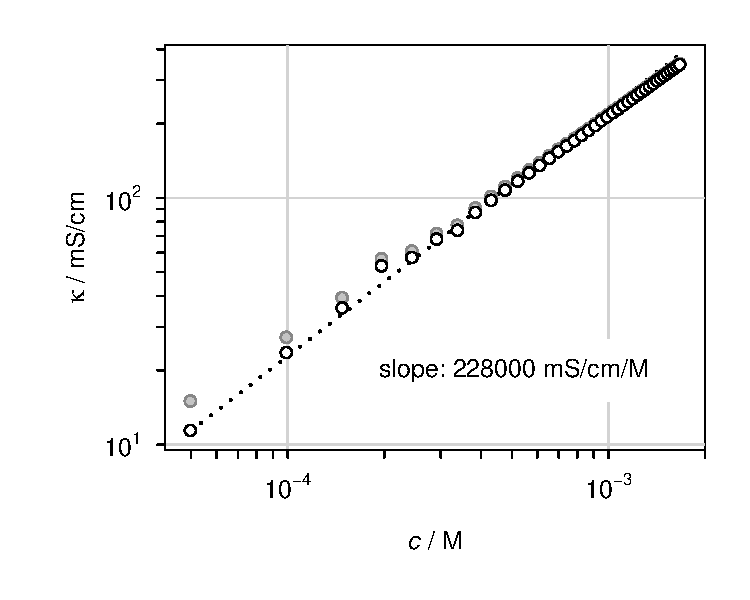
\includegraphics[width=.5\textwidth]{figures/plots/lfk_molar_1.pdf}
    \caption{Plotting the specific conductivity $\kappa$ against the concentration $c$ confirms the proportional relationship (dotted line), and thus legitimizes the consistency of the molar conductivity across the entire range of dilution. \\ The grey points show the raw conductivity recordings, the white points are corrected for the conductivity of the pure water. For further processing, the corrected values were used.}
    \label{fig:lfk_molar_1}
\end{figure}

\begin{figure}[H]
    \centering
    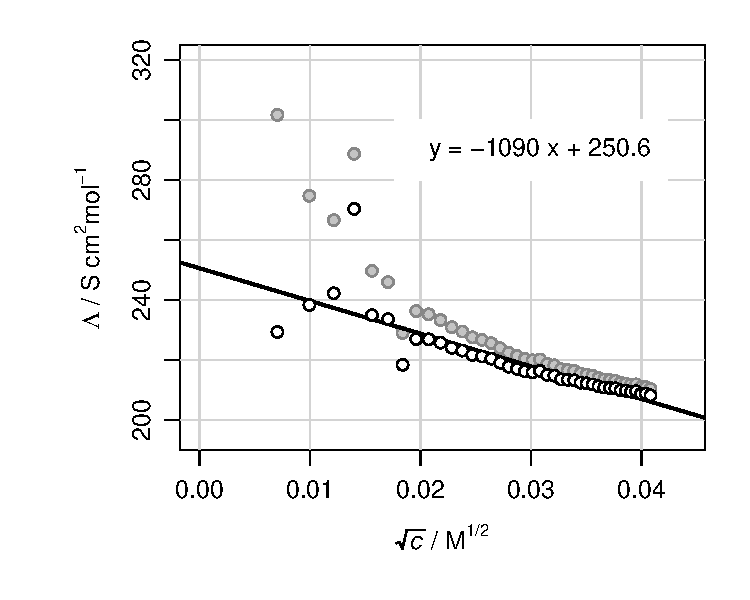
\includegraphics[width=.5\textwidth]{figures/plots/lfk_molar_2.pdf}
    \caption{Extrapolation to the limiting molar conductivity in accordance with \textit{Kohlrausch's square root law}. (Eq. \ref{eq:kohlrausch})}
    \label{fig:lfk_molar_2}
\end{figure}


\subsection{Conductometric titration}

\begin{figure}[H]
    \centering
    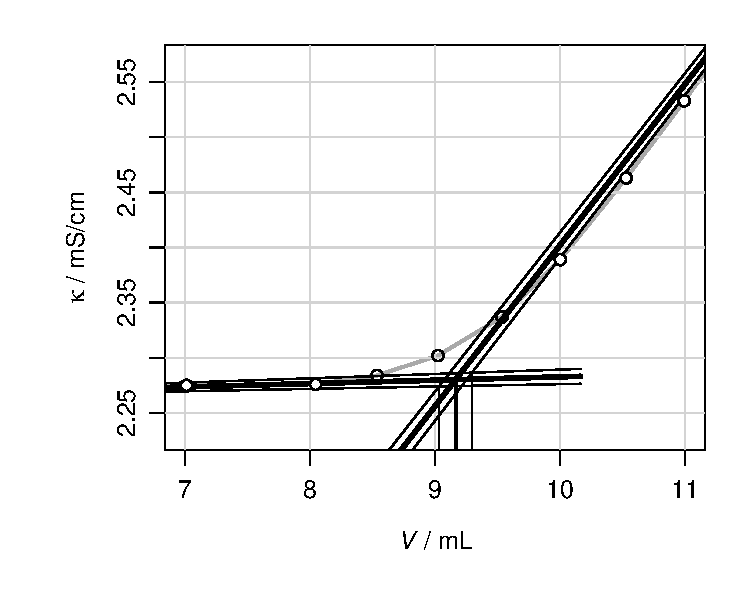
\includegraphics[width=.5\textwidth]{figures/plots/lfk_titration_zoom.pdf}
    \caption{Magnified view of the equivalence point in the titration of $\mathrm{K_2CO_3}$ with \qty[round-precision=5]{0.09997}{\M} $\mathrm{CaCl_2}$. The transparent points were not included in the calculation of the intersection point. The full titration plot can be seen in the appendix.\ref{fig:lfk_titr_full}}
    \label{fig:lfk_titr_zoom}
\end{figure}

\columnbreak

Intersecting the lines before and after the equivalence points of the conductometric titration (where $\kappa_1(V_{\mathrm{pre}}) = \kappa_{\mathrm{post}}(V_t)$) yields a titer volume $V_t =$ \qty{9.2 \pm 0.3}{\milli\litre}, which corresponds to an initial concentration of \qty{9.2 \pm 0.3}{\milli\M} of the $\mathrm{K_2CO_3}$ solution. The uncertainty interval was derived with the formula
\begin{equation}
    c_{\mathrm{\overline V_t}} = 2 * 
    \frac{s_{\mathrm{\overline V_t,post}} + s_{\mathrm{\overline V_t,pre}}}{a_{\mathrm{\kappa,post}} - a_{\mathrm{\kappa,pre}}}
\end{equation}

\iffalse{


%hi wie gehts voran? :)
%sameeeeeeee ich muss noch die leitfähigkeitstitration schrieben, dann bin ich fertig mit experimental, bis auf die chemikalien, da könnte ich eventuell kurz deine hilfe benötigen ( : 0 heiligenschein emojiiiiii) ah so geht das hahahha wenn man das verkehrt herum anscaut ist es ein orang utan mit offenem mund hahaha HAHAHAHAHAHAHAH
% :party-emoji:
% salut, ça va ?
% jetzt komm ich langsam in den Flow :)
% 

%
% (==)
% .  .
% -__-
% hahahah HA hahahhahah na gut, aber dann schau ich mal, dass ich das schnell fertig bekommen hihi und dann schau ich nochmal vorbei
% well das sieht eher aus wie ne creepy Katze... (holy cat!)
% ich hoffe auch dass ich das Zeugs in 1h fertig kriege. Dann kann ich gerne bei dir mithelfen :)
% :)))))))) dankööö boah diese reports kacken mich so an, unfassbar haha, so unnnnnnnötig, weil wir nix spannendes gemacht haben :*( so wenns wenigstens eine synthese gewesen wäreeeeeeee

% honestly bin ich froh um die Abwechslung vom AC Lab hahaa. Dort sind die Auswertung sooooo ööööde. Hier lerne ich irgendwie mehr finde ich.
%ok, das stimmt auch widerum haha
%\newpage
%hi hihihihihi weißt du zufälligerweise noch, welche chemicals wir in welchem experiment verwendet haben? 
% hmmmmmmm hahaha cry crycrycrycrycry . lemme see... dontcryeverythingwillbeok :) :))
% fotografiert habe ich: sodium carbonate, potassium carbonate, die fotos hast du mir schon geschickt :))
%im buch ist nämlich der graph mit sodium chloride und calcium chloride
% wollen wir mal im chat fragen?
%guter plan 
%soll ich machen?
% ooOOOOHHHH WAIT, MAN MUSS JA NUR INS LAB JOURNAL SCHAUN! :D XD
% Temperaturabhängigkeit: K2CO3hä wie hast du das jetzt da rausgelesen lol hahahahahaha
% weil ich aufgeschrieben hab dass ich 138.91 g K2CO3 eingewogen hab :)
% UUUUUUNNNNDDD molar conductivity steht m(Na2CO3) = 0.5298 g
% uuuuuunnnnd bei der Titration hatten wir ja die vorgefertigte Lösung K2CO3

%ich hab im excel stehen, dass wir molar mit beiden gemacht haben und konzentrationsabhängigkeit nur mit natrium

% ahjaaaa omg Janosch kann einfach nicht lesen
% eine Zeile darüber ssteht noch K2CO3 :see-no-more-monkey:cryyyyyyyyyyyyyyyyyyyyyyyyy omg wie wisssen wir einfach gar nix mehr von dem lab....? bei ddr wusste ich noch alles :(
% jaaa aber es war auch fürchterlich stressig und nichts wurde kommuniziert von den Assistenten. Ich mag mich nicht mal mehr erinnern bei wem wir das Experiment gemacht hatten, hätte die nicht eine E-Mail geschrieben hahahaha
%hahahhahaha
%aber was ist jetzt mit kso3?? hooppla C statt S. =>K2CO3 <=
% mannomann ich brauch eiine Pause... geh jeztt was essen.
%tu das ahahhaha ich glaub wir haben einmal abgewogen und dann einfach mit wasser aufgefüllt fürs nächsste experiment, damit die konzentration sich verändert... aber bin mir nicht mehr sicher welche chemikalie wann das erste mal verwendet wurde.... haben wir einen vorlage bericht für lfk?? OMG ICH WEISS ES WIEDER

\subsection{Density and refractive index}

The refractive index and density of acetone were measured at 

$n_D^{20} =$ \qty{1.35867}{1} and 

$\rho = $ \qty{0.7913}{\density} (\textit{method B}) 
\\and the density of acetone was calculated (\textit{method A}) to be 

\qty{0.7904 \pm 0.0026}{\density} 
\\corresponding with literature values of 

$n_D^{20} =$ \qty{1.3588}{1} and 

$\rho = $ \qty{0.7899}{\density}. \cite{meister} 
\\For n-hexane values of 

$n_D^{20} =$ \qty{1.37506}{1} and 

$\rho = $ \qty{0.6594}{\density} (\textit{method B}) and 

$\rho = $ \qty{0.6572 \pm 0.0022}{\density} (\textit{method A}) 
\\were obtained compared to literature values of 

$n_D^{20} =$ \qty{1.3751}{1} and 

$\rho = $ \qty{0.6603}{\density}. \cite{meister} 
\\It can be observed, that the results obtained for acetone are more precise than those of n-hexane. This could be explained for example by the varying grades of purity (99.5\% vs. 95\% specified by their producers.
\begin{figure}[H]
    \centering
    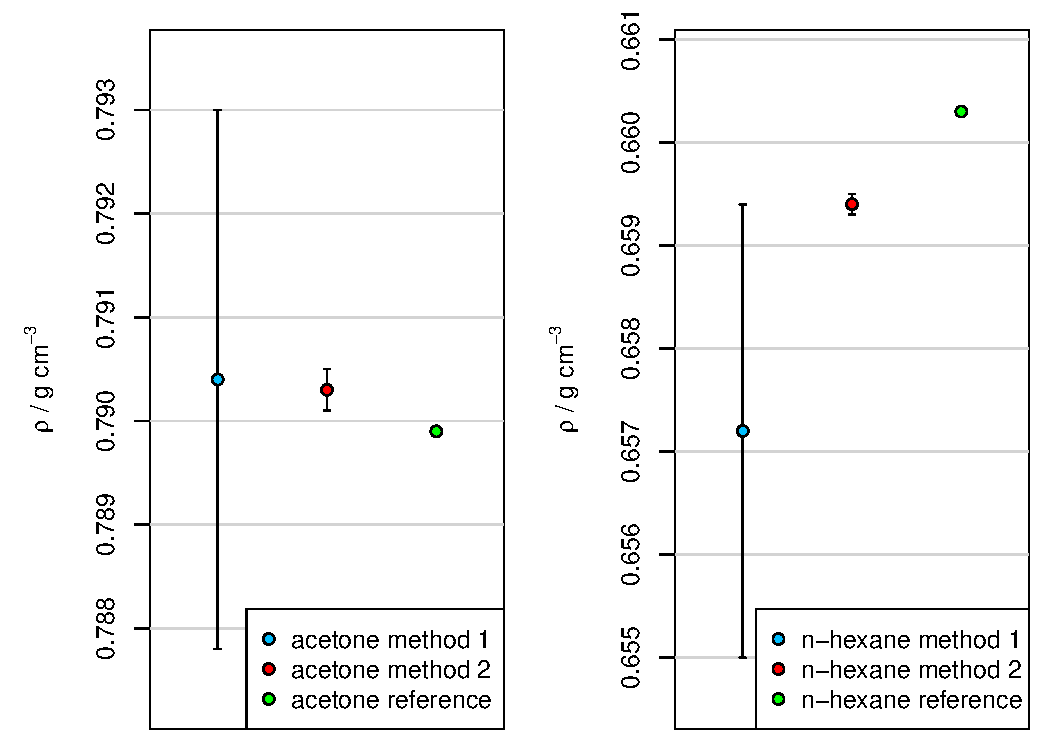
\includegraphics[width=.5\textwidth]{figures/rho-comparison.pdf}
    \caption{Comparisons of the density values measured, and reference values found in literature \cite{meister}.}
    \label{fig:rho_comp}
\end{figure}


\subsection{Vapor Pressure}

\begin{figure}[H]
    \centering
    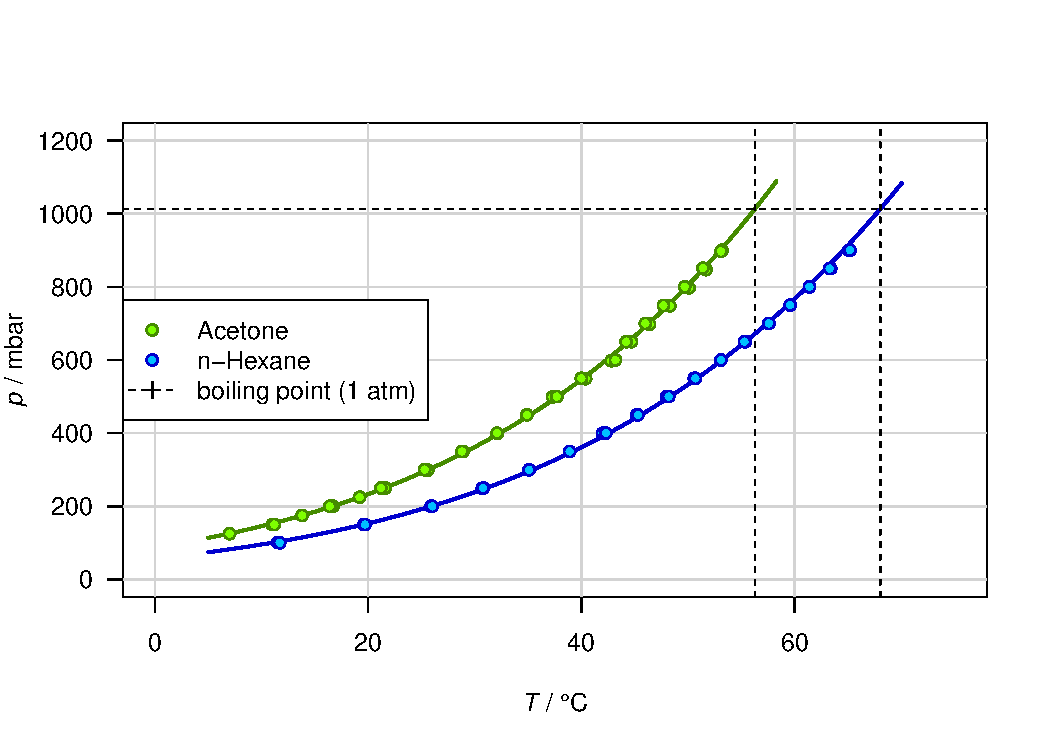
\includegraphics[width=.5\textwidth]{figures/DDR1_t_p.pdf}
    \caption{The vapor pressure curves illustrate the exponential correlation between vapor pressure and temperature. (Standard boiling points extrapolated and marked by the vertical and horizontal lines.)}
    \label{fig:ddr1_t_p}
\end{figure}

As mentioned in the introduction, vapor pressure can be described as $p(T)$. Accordingly, the results obtained from measuring the samples' boiling temperatures at differing surrounding pressures were plotted in a $p$-$T$-diagram, presented in Fig. \ref{fig:ddr1_t_p}.

Enthalpies of vaporization were calculated with by plotting logarithmic $\frac{p}{p_0}$ against inverse temperature $T$ via a linear regression model (Fig. \ref{fig:ddr1_inv_ln}) and calculating the slope $b$ of the resulting linear graphs. Expansion of equation (\ref{eq:6.2}) shows that it is equal to $\frac{\Delta_VH}{R}$. Results amounted to 

$\Delta_VH=$ \qty{32.49 \pm 0.26}{\kJpmole} for acetone and 

$\Delta_VH=$ \qty{32.66 \pm 0.25}{\kJpmole} for n-hexane. 
\\Acetone is a polar solvent and n-hexane is not. Because of this, one would assume, that its enthalpy of vaporization and standard boiling temperature would be higher than those of n-hexane because of stronger intermolecular bonds. Evidently, this is not the case. A possible explanation could be that though it is polar, acetone has a lower molar mass than n-hexane, meaning it would take less  energy to bring one mol of acetone from its fluid to its gaseous form than one mol of another substance with similar polarity.

 
\begin{figure}[H]
    \centering
    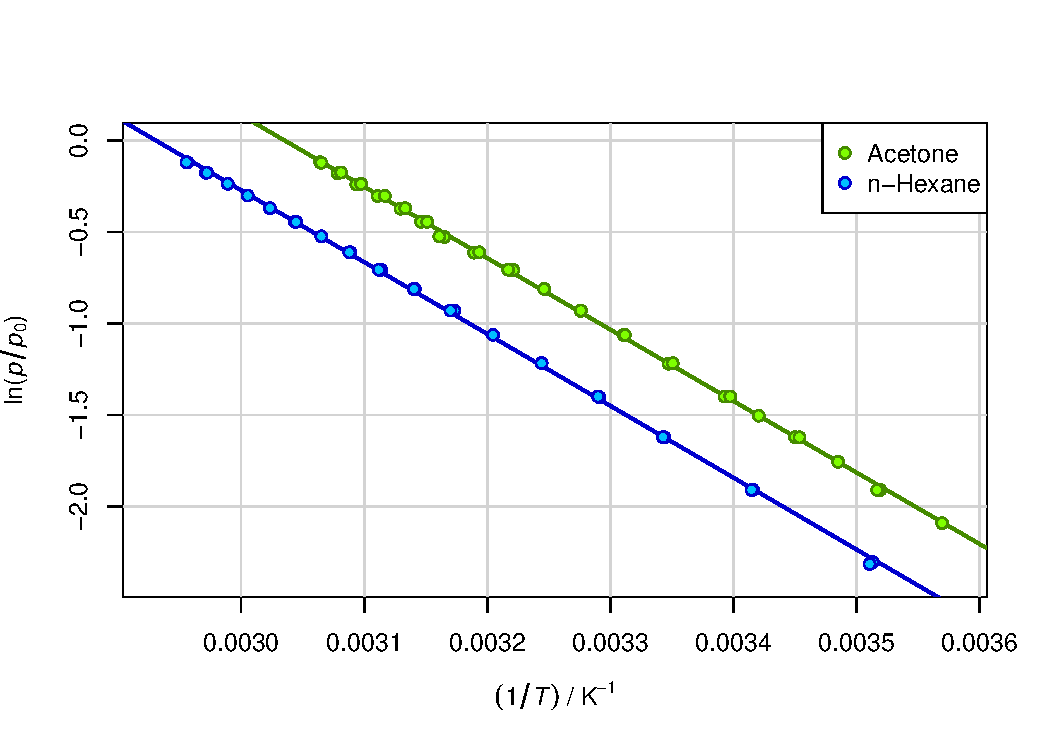
\includegraphics[width=.5\textwidth]{figures/DDR1_inv_ln.pdf}
    \caption{The Enthalpy of vaporization for each sample can be visualized in a $\ln\left(\frac{p}{p_0}\right)$ - $\frac{1}{T}$ diagram, because it is directly proportionate to the linear graph's slope $b$ (by factor of the gas constant $R$.)}
    \label{fig:ddr1_inv_ln}
\end{figure}


Normal boiling temperatures $T_0$ and standard entropies $\Delta_VS(T_0)$ of vaporization were also calculated with the help of the linear model parameters intercept $a$ and slope $b$ and found to be 

$T_0^{\text{acet}}$ = \qty{56.29}{°C}  

$T_0^{\text{nhex}}$ = \qty{68.06}{°C}
\\corresponding to literature values of 

$T_0^{\text{acet}}$ = \qty{56.15 \pm 0.3}{°C} 

$T_0^{\text{nhex}}$ = \qty{68.75 \pm 0.3}{°C}

and

$\Delta_VS(T_0)^{\text{acet}}$ = \qty{98.62}{\joule\per\mole\per\kelvin}

$\Delta_VS(T_0)^{\text{nhex}}$ = \qty{95.74}{\joule\per\mole\per\kelvin}.





\subsection{Transient evaporation cooling}
The data files generated by the \texttt{TREVAC} apparatus were imported to R. With the \mintinline{R}{identify()} command, the relevant time ranges for the peak integration could be selected graphically. (Fig. \ref{fig:nhex_peaks}) This data, including statistical parameters were then exported to a \textit{csv} file for documentation purposes and for further processing. To calculate the final values, including standard errors, a Jupyter notebook \cite{IPython:2007} with the \texttt{METAS UncLib} uncertainty modeling software \cite{unclib} was used. Formula \ref{eq:6.18} was 

For acetone, \qty{30.2 \pm 2.8}{\kJpmole} was calculated, and for n-hexane, \qty{32.0 \pm 1.9}{\kJpmole}, was found.

\begin{figure}[H]
    \centering
    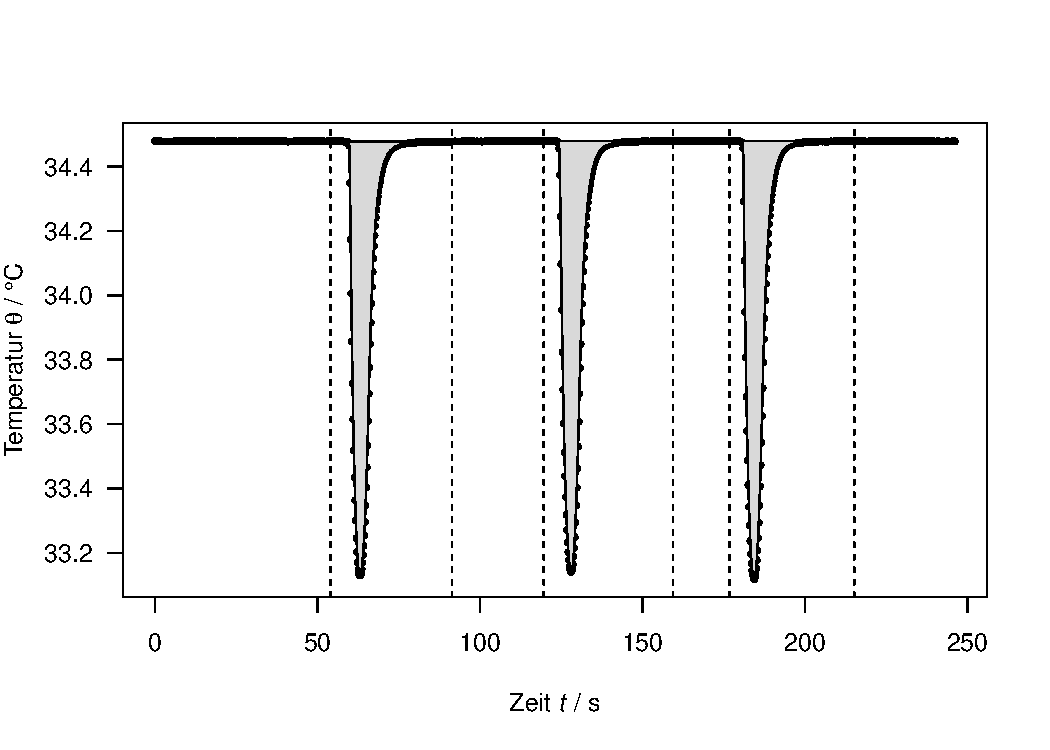
\includegraphics[width=.5\textwidth]{figures/n-hexane.pdf}
    \caption{Temperature peaks caused by n-hexane withdrawing heat from the measurement surface. The grey area is directly correlating with the enthalpy of evaporation $\Delta_VH_{\text{subst}}$ of the substance.}
    \label{fig:nhex_peaks}
\end{figure}

Standard values for $\Delta_VH$ can be found on the website of the \texttt{National Institute of Standard Technology}:

$\Delta_VH^0_{\text{acet}}$ = \qty{31.27}{\kJpmole} \cite{NIST:acet}

$\Delta_VH^0_{\text{nhex}}$ = \qty{31\pm 1}{\kJpmole} \cite{NIST:nhex}

}



            %hallihal
            %lo, kannst du vlt mal kurz im abstract deinen senf dazugeben hihi
            % top mach ich :) ? und gibts sonst noch etwas, dass ich noch machen könnte??
            % du hast dir glaub mal ne Pause verdient ;) du aber auch also wir machen das jetzt hier gemeinsam fertig :) 
            %du sogar noch mehr ich hab bei dem jetzt so wenig gemacht :( => Du hast die ganze Introduction und experimental super gut geschrieben! UUuuuund die superduperawesomemegawunderschönen Grafiken gezeichnet :)  Ich bin wirklich richtig fan davon. Kann ich dich dann mal anstellen für meine Bachelorarbeit? ;) hahahahahahaah danke :)))) ja klar... aber das ist ja nicht der anspruchsvolle teil gewesen (cry :*(, den hast du gemacht mit dem Auswerten und verstehen und ausrechenn und interpretieren.... wenn ich ehrlich bin, hab ich überhaupt keine ahnung, was unsere results bedeuten hahahhahaha. Tbh gibts da glaub auch nicht so viel tiefere Bedeutung hihi. Wir haben einfach Werte erhalten, die einigermassen mit dem der anderen übereinstimmt, aber doch ziemlich Schwankungen aufzeigt. Aber besser als bei Lilian und Aniko, die waren bei einem Wert um Faktor 10 daneben uuuupsiii. HAHAHAHAHAA, das wär mir saaaaafe auch passiert  ironischerweise hat es für einen der Werte (glaub K2CO3) gestummen, aber für NaCO3 nicht :clown-face: lol haha bzw. nicht-lol hahaha  egalllllllllllll alles nicht so wichtig :) 
        
        %YOLOOOOO hahahahahaha ja
        % alors, ich geh mir jetzt schnell Wasser holen, dann schau ich mir das Abstract an. Ich habe übrigens noch eine kleine Änderung gemacht in der Introduction. Siehe Kommentar :)
        % Der Rest sollte soweit stehen, abgesehen von den Übungen. Die Kap. Introduction/Experimental/Results/Discussion hatte ich vorhin nochmals durchgekämmt, sind 96% perfekt ;) yayyyyyyyy, ich hab auch noch paar sachen vorhin schon korrigiert, wir sollten zb darauf achten, dass die groß und kleinschreibung in den überschriften einheitlich ist.... ah oke, dann ists perfekt, so hätt ichs auch gemacht, aber hab ein paar große gesehen und dann hab ihs quasi falsch korrigieret
    % ich hatte bei mir jetzt auch alles klein korrigiert, weil gross irgendwie kacke aussieht hahaha -- tu mal neu rendern, dann solltes alles einheitlich sein :sonnenbrille-emoji: => :janosch-geht-wasser-holen-emoji: :zwinker-emoji:

%perfectttttt, wenns oke ist, könntest du da noch die werte einfügen einfach, es ist echt nix tolles, wirklich das bare minimum, weil mein hirn ist schon matsch ahha -- ohjee! Dann gönn dir wirklich mal eine kurze Pause. Aufstehen, dehnen, 2x ums Haus rennen (seriously), ...
        % alles eine Frage der Perspektive....
        % für mich ist das Programmieren viel gemütlicher hahahah :)))))) du genie aber deal, bei der bachelorarbeit mach ich dir hammer grafiken und du hilfst mir hammer graphen zu machen hehe, team work makes the dream work <3 <3 <3



        
        % well, ich hatte ja zuvor schon einiges an pause mit rennen, essen, im (kalten!) Brunnen baden gehen... hahaha booooooooah das klingt so nice (schmelzemojiiiiii)
        
        %\section{Conclusion}
        
            %
BLABLA

\iffalse{
The experiment was divided in three parts. The first two consisted of two different methods to determine the vaporization enthalpy and entropy of Cyclohexane and 1-Propanol. The first method was by measuring the boiling temperature at different pressures. For the second method the transient vaporization cooling was measured with the TREVAC-Apparatus provided by the ETH. Both methods turned out to be accurate, however the second one provided more accurate results which must have been due to the better thermometer which had a way smaller uncertainty. \\

The third part was the verification of Cyclohexane and 1-Propanol by measuring their densities and refraction indices. The density was once measured the naive way by weighing a known volume and once with a very expensive density measuring device. The second method delivered very accurate results, whereas the first was just a bit off the literature values but still good. The refraction indices were also measured by a device which directly gave back the correct values.
}
        
        % References
        %\input{References.bib}
        \printbibliography[
            heading=bibintoc,
            title={References}
        ]

        
    \end{multicols}
    \newpage
      
    \appendix
    \section{Appendix}

        \section{Coursebook exercises}

\subsection{Ion velocity}

Using equation \ref{eq:7.4}:

\begin{equation} \label{eq:7.4.ex}
    v_i = \frac{e E}{6 \pi \eta} \frac{z_i}{r_i}
\end{equation}

yields $v_{\mathrm{Mg^{2+}}} =$ \qty{1.70}{\micro\meter\per\second} and $v_{\mathrm{CH_3COO^{-}}} =$ \qty{0.85}{\micro\meter\per\second}.

$\mathrm{Mg^{2+}}$ moves faster than $\mathrm{CH_3COO^{-}}$ due to its higher charge (and smaller size, which is not even taken into account in this exercise). A speed of micrometers per second seems small at first glance, but is really fast compared to the ions size and the density of particles in a liquid.




\subsection{Molar conductivity of pure water}

$$\Lambda \approx \Lambda^0 = \lambda_+^0 + \lambda_-^0 = \qty{547}{\Smolar}$$

$$pH = 7 \implies [H^+] = \qty{1e-7}{\mole\per\liter}$$

$$= \qty{1e-10}{\mole\per\centi\meter\cubed}$$

$$\kappa = \Lambda c = \qty{547}{\Smolar}\qty{1e-10}{\mole\per\centi\meter\cubed}$$

$$= \qty{5.47e-8}{\siemens\per\centi\meter}$$



\subsection{Spagetthi water}

$$\qty{8}{\gram} \text{ NaCl in water } \widehat{=} 0.137 \text{ } \unit{\mole\per\liter} = \qty{137}{\mole\per\centi\meter\cubed}$$

$$\Lambda \approx \Lambda^0 = \lambda_+^0 + \lambda_-^0 = \qty{127}{\Smolar}$$

$$\kappa = \Lambda c = \qty{127}{\Smolar}\qty{137}{\mole\per\centi\meter\cubed}$$

$$= \qty{0.928}{\siemens\per\centi\meter}$$



\subsection{Limiting molar conductivity HCl and KOH}

$$\Lambda^0_{\mathrm{HCl}} = \lambda_{\mathrm{H^+}}^0 + \lambda_{\mathrm{Cl^-}}^0 = \qty{426}{\Smolar}$$

$$\Lambda^0_{\mathrm{KOH}} = \lambda_{\mathrm{K^+}}^0 + \lambda_{\mathrm{OH^-}}^0 = \qty{271}{\Smolar}$$

The calculated values are slightly higher than those extrapolated in Fig. 7.4 of the coursebook. 




\subsection{Reading the titration curve}

$V_t = \qty{18.30 \pm 0.25}{\milli\liter}$

$\widehat{=} \qty{1.800 \pm 0.025}{\milli\mole}$

$\widehat{=} \qty{0.249 \pm 0.003}{\gram}$

%alles abgecheckt von meiner seite aus :)
% yayyy!! und du hast wieder Zugriff :D

        
\subsection{R-Scripts} \label{r_scripts}

\subsubsection{Vapor Pressure Analysis}
\Rfile{scripts/DDR1_shared_plot.R}
%\inputminted{R}{scripts/DDR1_shared_plot.R}
% \caption{Auswertungsskript Dampfdruckkurve}

\newpage
\subsubsection{\texttt{TREVAC} Analysis}
\Rfile{scripts/DDR2.R}


\newpage

\begin{figure}[H]
    \centering
    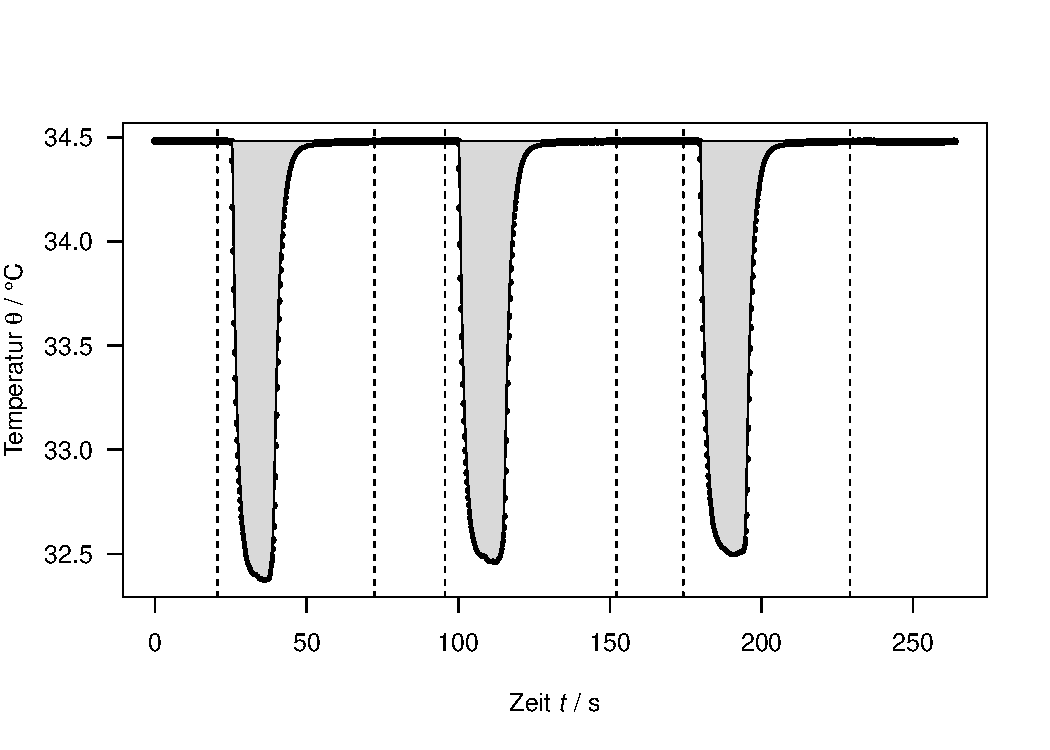
\includegraphics[width=.5\textwidth]{figures/methanol.pdf}
    \caption{\texttt{TREVAC} area analysis of methanol as reference value.}
    \label{fig:sketch_rho}
\end{figure}

\begin{figure}[H]
    \centering
    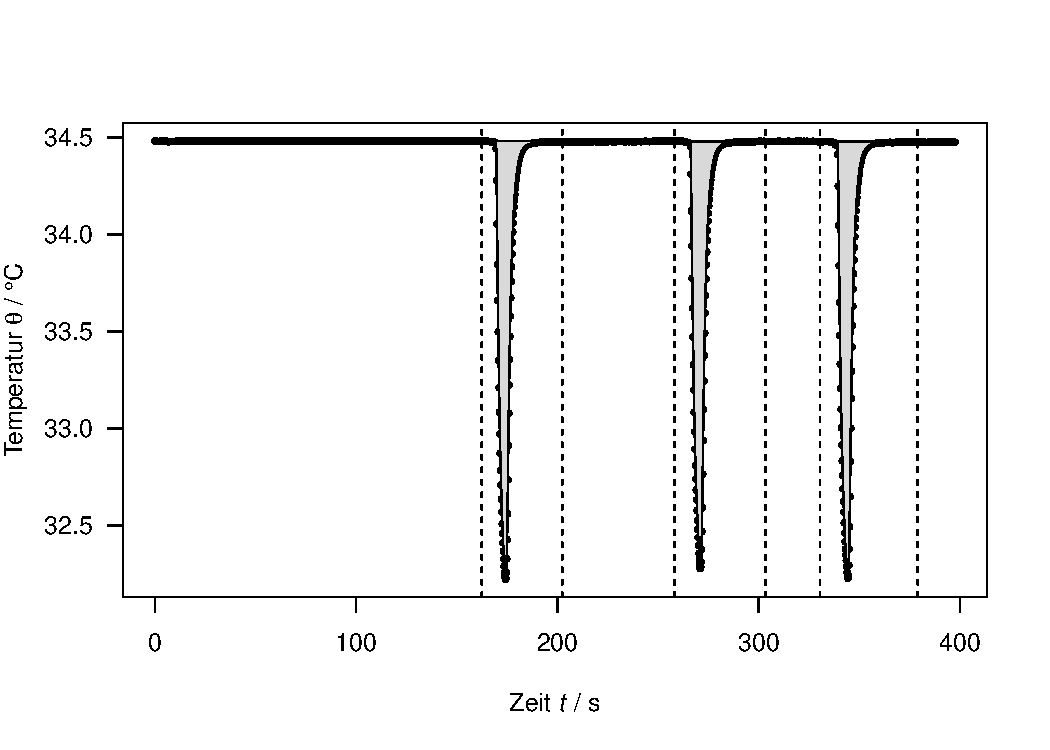
\includegraphics[width=.5\textwidth]{figures/acetone.pdf}
    \caption{\texttt{TREVAC} area analysis of acetone.}
    \label{fig:sketch_rho}
\end{figure}

\begin{figure}[H]
    \centering
    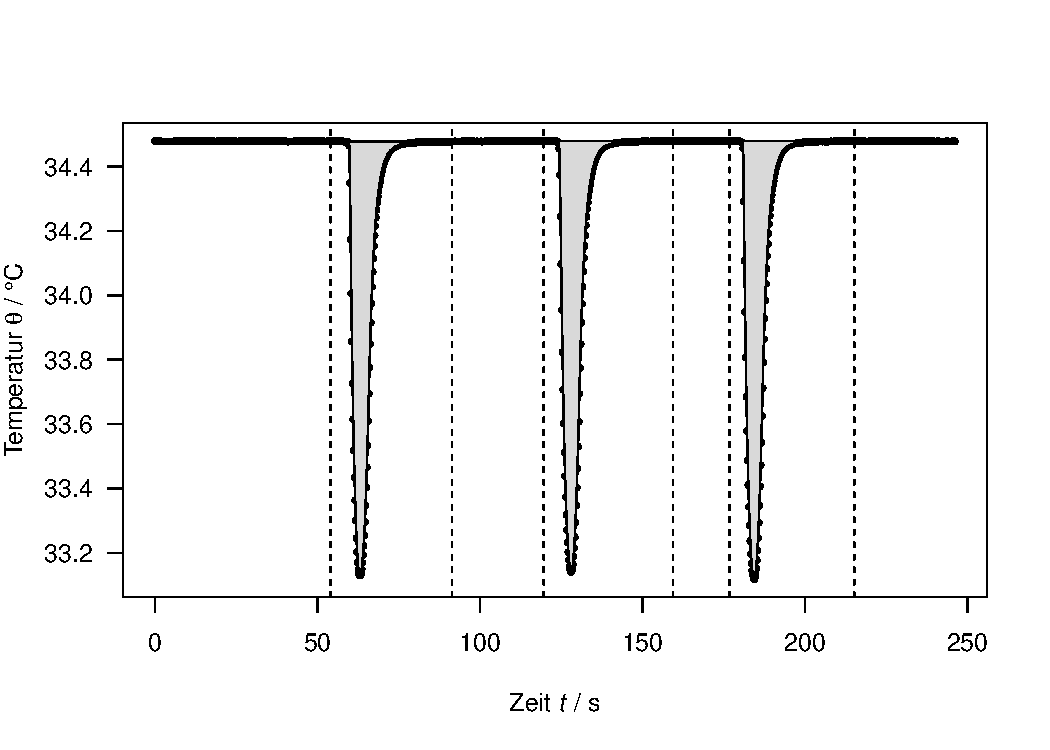
\includegraphics[width=.5\textwidth]{figures/n-hexane.pdf}
    \caption{\texttt{TREVAC} area analysis of n-hexane.}
    \label{fig:sketch_rho}
\end{figure}


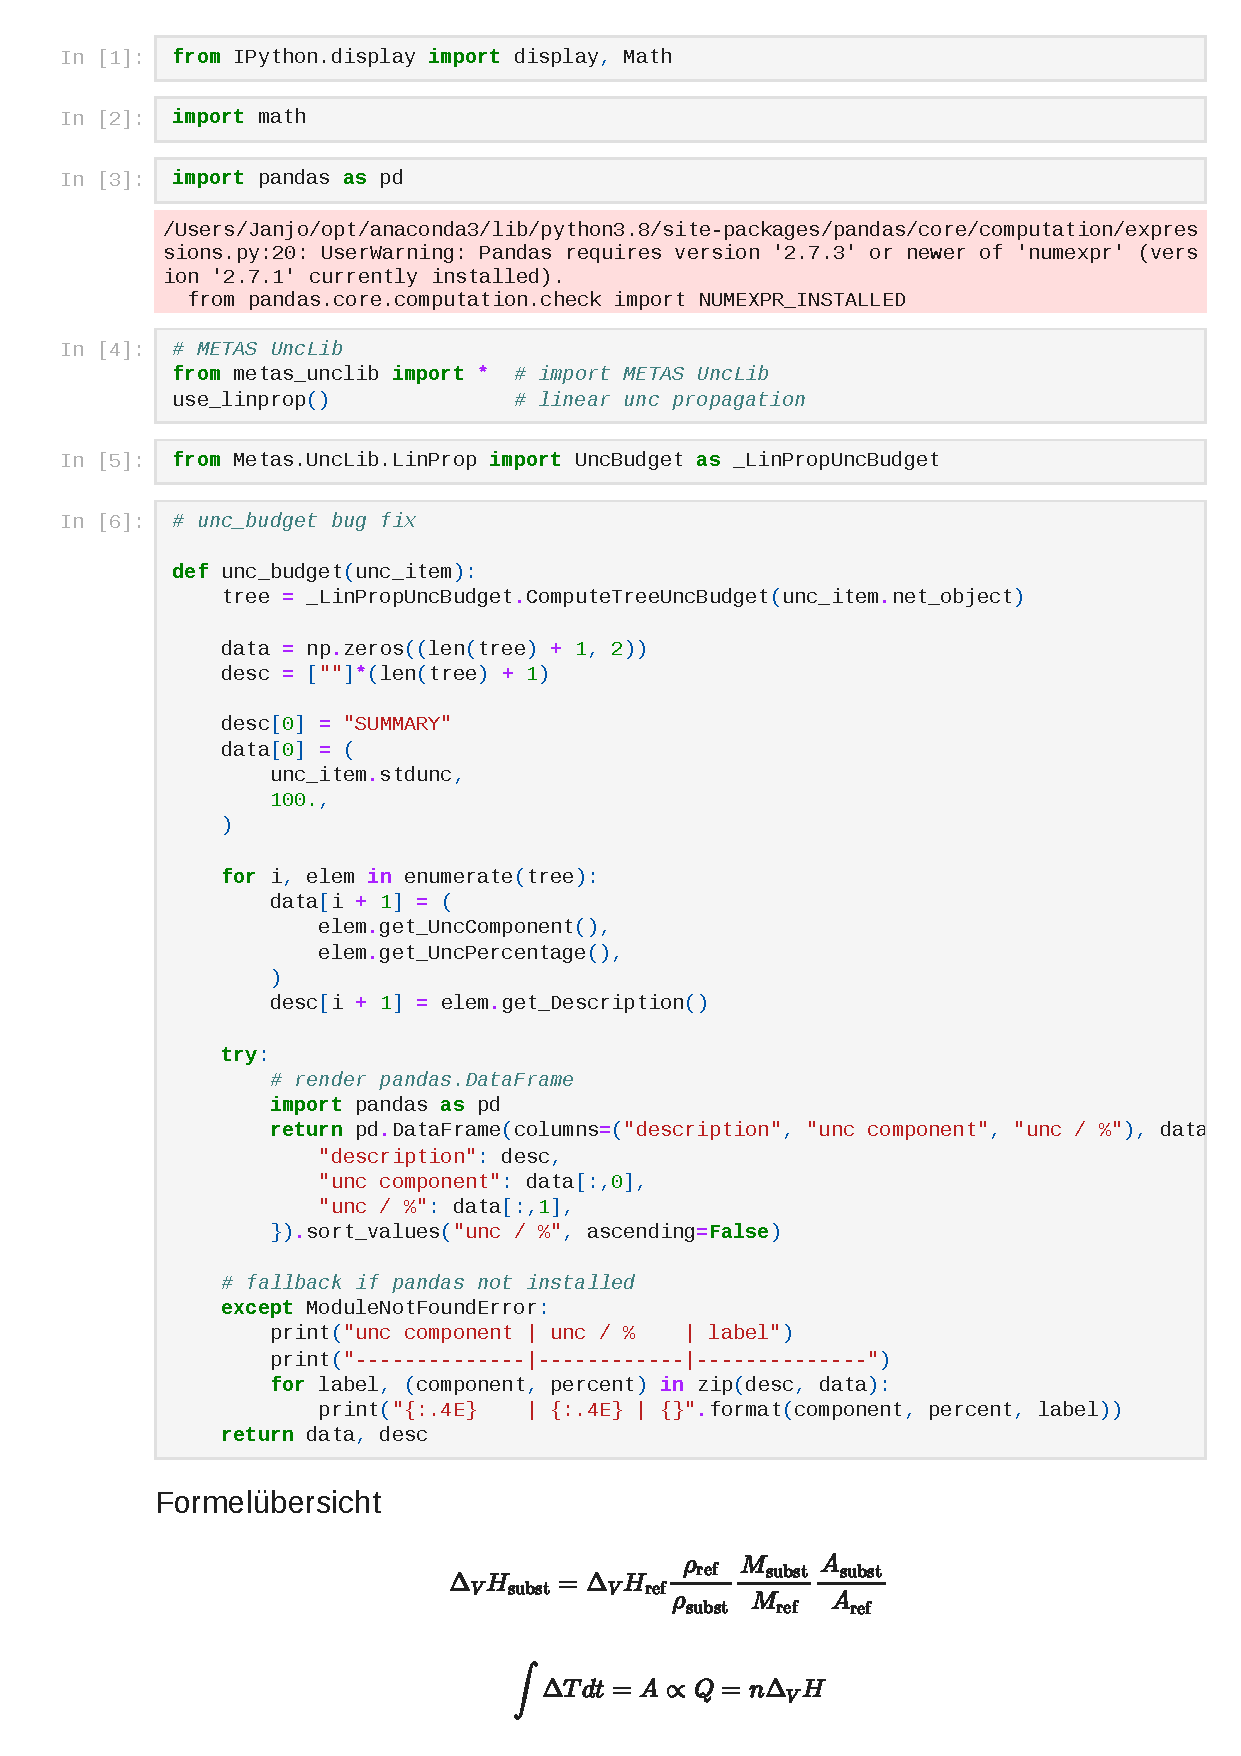
\includepdf[pages=1, scale = 0.75, pagecommand=\subsubsection{TREVAC results and uncertainty estimates}]{scripts/metas_unclib_ddr2.pdf} 
\includepdf[pages=2-, scale = 0.75,pagecommand={}]{scripts/metas_unclib_ddr2.pdf} \label{lab_journal}

\newpage
\subsubsection{Density comparison plot}
\Rfile{scripts/rho_comparisons.R}

\newpage
\subsubsection{Plotting helper scripts}
\Rfile{scripts/helpers.R}

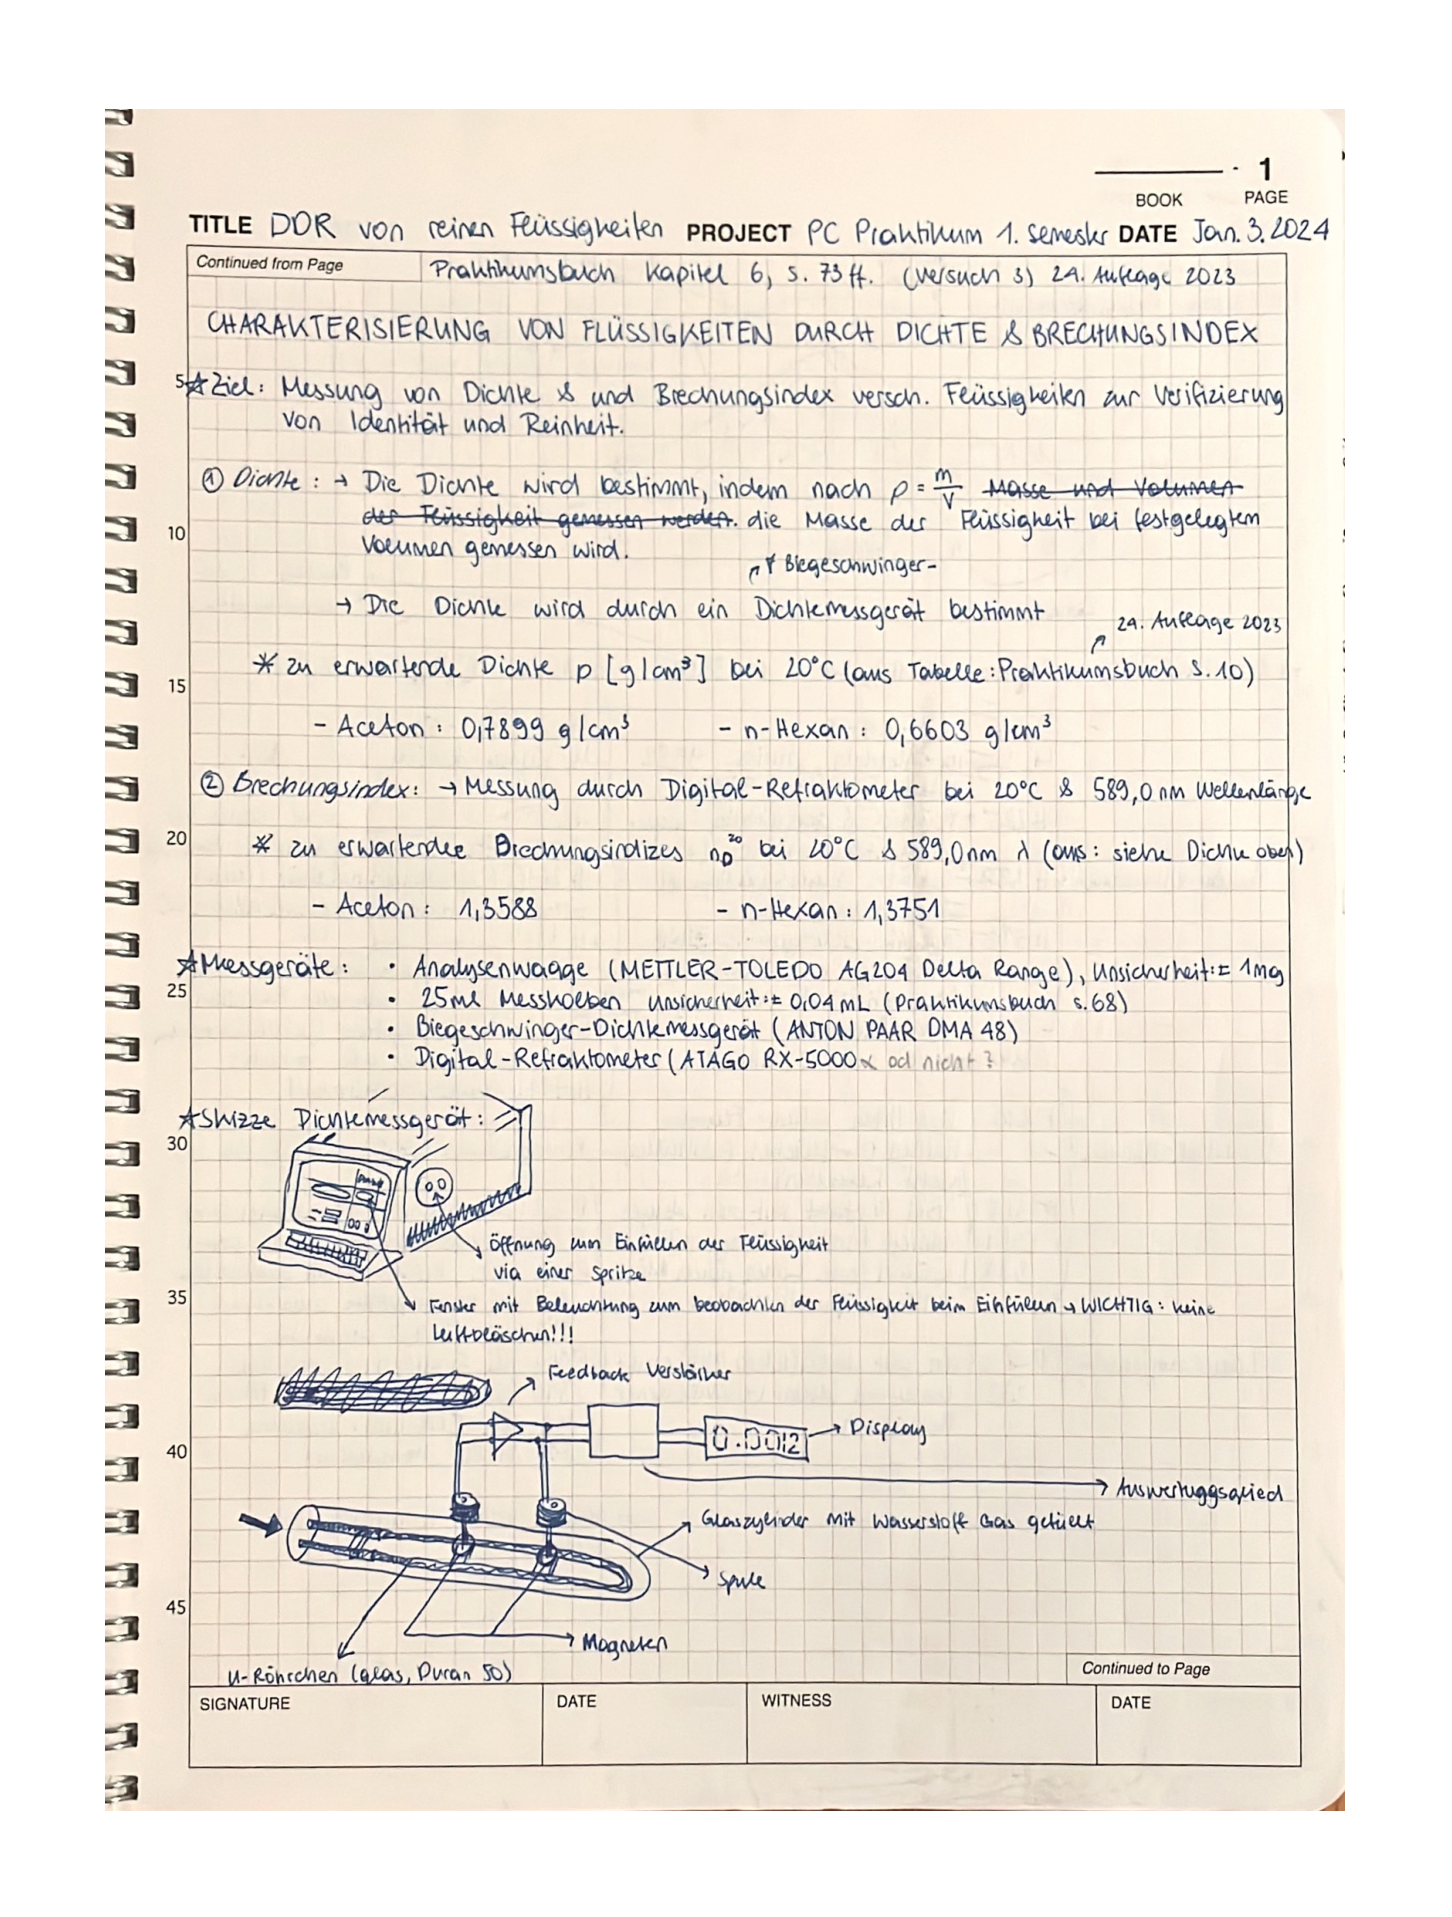
\includepdf[pages=1, scale = 0.75, pagecommand=\subsection{Lab Journals}]{figures/ddr_lab_journal.pdf} 
\includepdf[pages=2-, scale = 0.75,pagecommand={}]{figures/ddr_lab_journal.pdf} \label{lab_journal}


\iffalse{
\lstinputlisting[caption=Automatic rounding functions to fit the 25 rule of the significant digits.]{scripts/25Utils.R}
\lstinputlisting[inputencoding=utf8/latin1, caption=Code for the evaluation of the first experiment: Enthalpy of evaporation.]{scripts/DDR.R}
\lstinputlisting[inputencoding=utf8/latin1, caption=Code for the evaluation of the second experiment: Transient evaporation cooling.]{scripts/DDR2.R} \label{ddr_code2}

\includepdf[pages=1, scale = 0.75, pagecommand=\subsection{Lab journal copies}]{figures/LabJournalDDR.pdf} 
\includepdf[pages=2-, scale = 0.75,pagecommand={}]{LabJournalDDR.pdf} \label{lab_journal}

\includepdf[pages=1, scale = 0.75, pagecommand=\subsection{Exercises from the script}]{figures/U_DDR.pdf}
\includepdf[pages=2-, scale = 0.75,pagecommand={}]{U_DDR.pdf}

\subsection{Additional data plots}

\subsubsection{Transistent evaporation cooling}

\begin{figure}[H]
    \centering
    \subfigure[]{\includegraphics[width=.49\textwidth]{figures/DDR2_cyc.pdf}}
    \subfigure[]{\includegraphics[width=.49\textwidth]{DDR2_pol.pdf}}
    \caption{Profile of the evaporation of 5 $\mu$L of (a) Cyclohexane and (b) 1-Propanol.}
    \label{fig:ddr2_appendix}
\end{figure}

\subsection{Safety}

The Hazards-\&Precautionary phrases were copied from data sheets found at \cite{Sigma-Aldrich}.

\subsubsection{Cyclohexane}
\ghspic[scale = 0.75]{flame} \ghspic[scale = 0.75]{acid} \ghspic[scale = 0.75]{exclam} \ghspic[scale = 0.75]{aqpol} \\

\noindent
\ghs{h}{225} \\
\ghs{h}{304} \\
\ghs{h}{315} \\
\ghs{h}{336} \\
\ghs{h}{410} \\
\ghs{p}{210} \\
\ghs{p}{233} \\
\ghs{p}{273} \\
\ghs{p}{301+310}\\
\ghs{p}{303+361+353}\\
\ghs{p}{331} \\

\subsubsection{1-Propanol}
\ghspic[scale = 0.75]{flame} \ghspic[scale = 0.75]{acid} \ghspic[scale = 0.75]{exclam} \\

\noindent
\ghs{h}{225} \\
\ghs{h}{318} \\
\ghs{h}{336} \\
\ghs{p}{210} \\
\ghs{p}{233} \\
\ghs{p}{240} \\
\ghs{p}{241} \\
\ghs{p}{280} \\
\ghs{p}{305+351+338}\\

\subsubsection{Methanol}
\ghspic[scale = 0.75]{flame} \ghspic[scale = 0.75]{skull} \ghspic[scale = 0.75]{health}

\noindent
\ghs{h}{225} \\
\ghs{h}{301}+\ghs{h}{311}+\ghs{h}{331} \\
\ghs{h}{370} \\
\ghs{p}{210} \\
\ghs{p}{233} \\
\ghs{p}{280} \\
\ghs{p}{301}+\ghs{p}{310} \\
\ghs{p}{303}+\ghs{p}{361}+\ghs{p}{353} \\
\ghs{p}{304}+\ghs{p}{340}+\ghs{p}{311} \\

}
    
    %\section{Acknowledgment}
        
        %
The authors would like to thank the team at DCHAB for enabling this programme.


\iffalse{
The authors would like to thank the ETH Zürich for providing them with the measuring infrastructure and support to be able to conduct the experiments. They would also like to thank Dr. Erich Christian Meister for spontaneously stepping in for their lab assistant when he could not attend due to sickness.
Additionally the authors would like to thank the open-source community for providing them with the software tools and techniques used for data analysis in the form of R.
}

\end{document}
